\documentclass[12pt]{article}   % you have 10pt, 11pt, or 12pt options

\usepackage{import}
\subimport{../}{setup.tex}


\begin{document}  % necessary part of document


\title{LaTeX \, Template and Tutorial for Math Modelers}
%\author{DO NOT INCLUDE YOUR NAMES!!!!!}
\date{\today}

\maketitle

\begin{abstract}
Your abstract or summary can go here.
\end{abstract}

\newpage

\tableofcontents

\newpage

\section{Introduction}

\vspace{1cm}

Here are some typesetting features you may want to use when writing up your classwork, or
the mathematics in your class summary. If you want to type a paragraph of text, simply
start typing.

To start a new paragraph, leave a blank line before the new paragraph.

\bigskip

Here's a bullet list of some of the math symbols you may need.  Note that any math
formulas must be surrounded by dollar signs, like so:  $H(s,t) = F(\alpha(s),t)$.  If you
surround a math formula by double dollar signs, your formula will be centered on a line by
itself, like so:
$$H(s,t) = F(\alpha(s),t).$$  Whatever you type afterwards will begin again on a separate line.

\begin{itemize}     % replace itemize with "enumerate" for numbered list
\item Greek letters:  $\alpha, \gamma, \pi, \tau$
\item product of two sets $X \times Y$
\item Intersections $\cap$, unions $\cup$, and disjoint unions $\sqcup$
\item {\it italics} and {\bf bold}
\item related to: $\sim$, homotopic to $\simeq$, and isomorphic to $\cong$
\item Fractions which fit inside a paragraph of text:
$\frac{az + b}{cz + d}$,
and bigger fractions: $\displaystyle{\frac{az + b}{cz + d}}$
\item Subscripts and exponents:  $z_1$, $w^2$, $z_2^3$, $f_*(x)$,  $p^{-1}(b)$
\item Derivatives: $f'(x)$, integrals $\int_a^b f(x) \, dx$, % the \, adds a space between f(x) and dx
and limits $\lim_{n \rightarrow \infty} a_n$ or $\displaystyle{\lim_{n \rightarrow \infty} a_n}$
\item Not equals:  $c \neq 0$, or greater than / less than or equal: $c \ge 0$, $x \le 17$
\item functions defined in pieces:  $$p(x) =  \left\{ \begin{array}{ll}
                x & \mbox{for } x \in [0,1] \\
                x-1 & \mbox{for } x \in [2,3]
                \end{array} \right.$$
\item Left quotes `` and right quotes "
\item Composition:  $g \circ f$, and multiplication:  $g \cdot f$
\item Left and Right Set Brackets need a backslash:  $\{x : p(x) = b\}$
\item Is an element of: $b \in B$
\item $\R$,  $\Sph^2$, $\T^2$, $\Z$
\item To put a word in with a string of math symbols, use mbox:  $f \sim g \mbox{ rel } A$,
otherwise, it looks like: $f \sim g rel A$.
\item $p|_{\widetilde{U}}$
\item group presentation:  $\langle a,b : ab\overline{a} \rangle$
\item A lot of symbols you might want to know are just what you think
they might be, preceded by a backslash:  $\cos \theta, \not\in, \rightarrow, \mapsto,
\Leftrightarrow, \longrightarrow, \subset, \subseteq$
\end{itemize}


\noindent There are nice, pre-written environments for Theorems and Proofs,
as below:

\begin{theorem}{(Unique Path Lifting Property)}
% leave this as empty brackets : {} if theorem has no name
Here's where you type in the text of the theorem.
\end{theorem}

\begin{proof}
And this is where you type in the proof!
\end{proof}

\begin{lemma}
{} % this lemma has no name
Here's where you put the body of a lemma.
\end{lemma}

\bigskip

\noindent You might also want to write up the following things:

\begin{enumerate}
\item A numbered list,

\item or a sequence of equations, lined up at the equals sign...
\begin{eqnarray*}   % do not need dollar signs because eqnarray puts you in math mode
d(z_1,z_2) & = & \int_{z_1}^{z_2} \frac{1}{t} \, dt \\
& = & \ln(z_2) - \ln(z_1) \mbox{\hspace{1cm} by the Fund Thm of Calc}\\
& = & \ln\left(\frac{z_1}{z_2}\right) \\ % using \left( and \right) makes larger ()
\end{eqnarray*}

\item or some Commutative Diagrams...

$$\begin{array}{rcl}
\Sph^2  & \stackrel{g}{\longrightarrow} & \Sph^2 \\
\mbox{\footnotesize{S}} \downarrow & & \downarrow \mbox{\footnotesize{S}} \\
\R^2 & \stackrel{f}{\longrightarrow} & \R^2 \\
\end{array}$$

\item or a Table...

\begin{center}
\begin{tabular}{|c|c|}
\hline 
Column A & Column B \\ 
\hline
$T^2 \# S^2$ & $P^2 \# P^2$ \\
$K^2$ & $K^2 \# P^2$ \\
$S^2 \# S^2 \# S^2$ & $S^2 \# S^2$ \\
$P^2 \# T^2$ & $P^2 \# P^2 \# P^2 \# K^2$ \\
$K^2 \# T^2 \# P^2$ & $T^2$ \\
\hline
\end{tabular}
\end{center}

\item or a picture, such as in Figure \ref{fig:fun} (you will need to use a .eps graphics file for Windows, and a .pdf graphics
file for Mac).

\begin{figure}[h]
\centerline{\hspace{-1cm}
    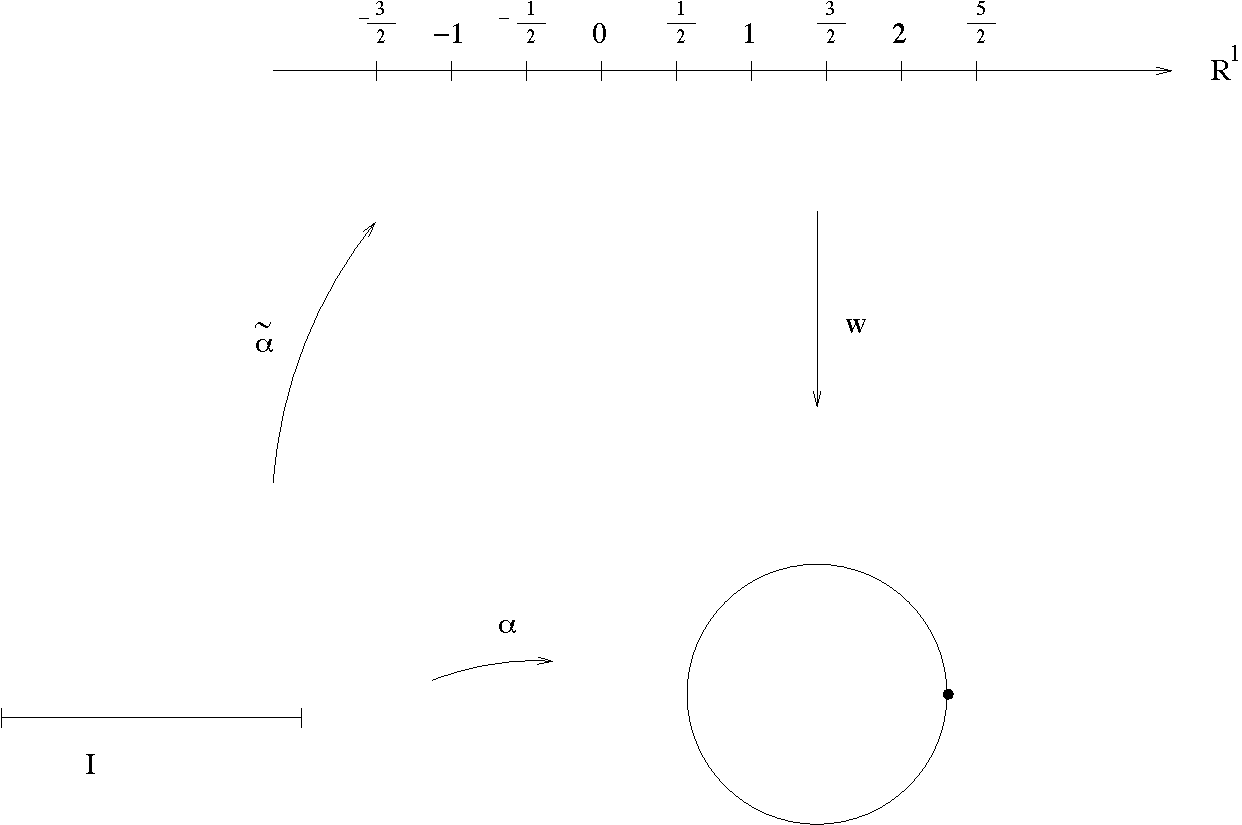
\includegraphics[height={6cm}]{resources/unwrapcircle.pdf}} 
    \caption{Lifting the circle to its universal cover}
\label{fig:fun}
\end{figure}


\item  ...and you can always ask me {\it before the contest starts} if you need to typeset something that I haven't
included here.
\end{enumerate}

\bigskip\bigskip

\begin{quote}
(You might want to save this document somewhere -- even just email it to yourself -- in
case some day you decide you want to use \LaTeX to typeset something else.)
\end{quote}


\newpage

\section{Now You Try It!}

\subsection{Assumptions}

For practice, type bullet list here

\subsubsection{Approach}

For practice, type a numbered outline of approach here

\section{The Model}

For practice, put a new picture here.

\section{Solutions}

For practice, type a few formulas here.

\section{Solution Comparison Methods}

For practice, type a table of data here

\section{Results}

\section{Conclusion - Strengths and Weaknesses}

\newpage %-----------------------------------------------------------------------------------------------------------

\begin{thebibliography}{99} % 99 is the highest number of references this expects;  this sets the expected width of the citation


\bibitem{Erdos01} P. Erd\H os, \emph{A selection of problems and
results in combinatorics}, Recent trends in combinatorics (Matrahaza,
1995), Cambridge Univ. Press, Cambridge, 2001, pp. 1--6.

\bibitem{ConcreteMath}
R.L. Graham, D.E. Knuth, and O. Patashnik, \emph{Concrete
mathematics}, Addison-Wesley, Reading, MA, 1989.

\bibitem{Knuth92} D.E. Knuth, \emph{Two notes on notation}, Amer.
Math. Monthly \textbf{99} (1992), 403--422.

\bibitem{Simpson} H. Simpson, \emph{Proof of the Riemann
Hypothesis},  preprint (2003), available at 
\url{http://www.math.drofnats.edu/riemann.ps}.

\bibitem{HB98} Huynen, M.~A. and Bork, P. 1998. Measuring genome evolution. {\em
Proceedings of the National Academy of Sciences USA}
  95:5849--5856.

\bibitem{CA} Caprara, A. 1997. Sorting by reversals is difficult. In: {\em
Proceedings of the First Annual International Conference on Computational
Molecular Biology (RECOMB 97),} New York: ACM.  pp. 75-83.

\bibitem{MSW00}McLysaght, A., Seoighe, C. and Wolfe, K.~H. 2000. High frequency
of inversions during eukaryote gene order evolution.     In Sankoff, D. and
Nadeau, J.~H., editors, {\em Comparative Genomics},  Dordrecht, NL: Kluwer
Academic Press. pp. 47--58.

\bibitem{Rei91} Reinelt, G. 1991. {\em The Traveling Salesman - Computational
Solutions for TSP Applications.} Berlin: Springer Verlag.

\end{thebibliography}

\end{document}

